%-----------------------------------------------------------------------------%
%                                                                             %
%    K A P I T E L   3                                                      %
%                                                                             %
%-----------------------------------------------------------------------------%

\chapter{Contact Stability Constrained DDP}\label{c3}
This chapter presents a generic method for integrating contact stability constraints into DDP-like solvers. The key idea is to define inequality constraints for unilaterality, friction and the \gls{CoP} of each contact surface with the goal of generating inherently balanced motions.

\section{The Idea}\label{sec:StabilityIdea}
Stability of the contacts is an essential objective of motion planning since prevents the robot from sliding and falling down. In \cref{sec:TheoryStability} we have explored two different criteria for ensuring contact stability for dynamic systems, namely the \gls{ZMP} and \gls{CoP}. As outlined, the application of the \gls{ZMP} is limited due to the assumptions of sufficiently high friction and the existence of one planar contact surface. Since we want to provide a \textit{generic} method that can also be used for e.g. walking up stairs, these simplifying assumptions do not hold anymore. 

Consequently, we decide to model a 6D surface contact, as introduced in \ref{eqn:EoMLeggedRobotSurfaceContact} with dedicated constraints for (i) unilaterality of the contact forces (ii) Coulomb friction on the resultant force, and (iii) \gls{CoP} inside the support area. For the sake of simplicity, we model a rectangular contact area. Nevertheless, this concept can be extended  to arbitrary feet designs. This approach can be compared to the concept of contact wrench cone \cite{caron2015stability}, without additionally enforcing the yaw torque constraint. These inequality constraints for surface contacts can compactly be summarized as
\begin{subequations}\label{eqn:contractWrenchConeReduced}
\begin{align}
f_i^z &> 0 \label{subeqn:stabilityUnilaterality},\\
\mid f_i^x\mid &\leq \mu f_i^z \label{subeqn:stabilityFrictionX},\\
\mid f_i^y\mid &\leq \mu f_i^z \label{subeqn:stabilityFrictionY},\\
\mid X\mid & \geq C_x \label{subeqn:stabilityCoPPitch},\\
\mid Y\mid & \geq C_y \label{subeqn:stabilityCoPRoll}.
\end{align}
\end{subequations}
%Original CoP constraints from Caron paper for horizontal floor
%\mid \tau_i^x\mid & \leq Yf_i^z \label{subeqn:stabilityCoPPitch},\\
%\mid \tau_i^y\mid & \leq Xf_i^z \label{subeqn:stabilityCoPRoll}.

Let us now detail each line of the approach. 
The first inequality \cref{subeqn:stabilityUnilaterality} accounts for the unilaterality of the contact force. By nature, contact forces always have to be positive since the robot can only \textit{push} from the ground, not \textit{pull} to the ground (\cref{img:simple_contact}). 
Inequality \cref{subeqn:stabilityFrictionX,subeqn:stabilityFrictionY} corresponds to the Coulomb friction, where $\mu$ denotes the static coefficient of friction. From a modeling perspective, this can be interpreted via the concept of spatial friction cones \cite{kao2016contact}. If, and only if the distributed contact forces lie inside their respective friction cones, these constraints are satisfied. 
Finally, inequality \cref{subeqn:stabilityCoPPitch,subeqn:stabilityCoPRoll} constrain the \gls{CoP} to lie inside the rectangular contact area of each foot (see \cref{img:contact_surface}). $C_x$ and $C_y$ denote the x and y position of $\bp_{CoP}$, respectively. These \gls{CoP} constraints prevent the robot from tilting around the edges of the rectangular surface contact. In particular, \cref{subeqn:stabilityCoPPitch} corresponds to a constraint of tilting around the pitch axis and \cref{subeqn:stabilityCoPRoll} prevents tilting around the roll axis.

Both, the unilaterality of the contact forces and the friction cone constraints, are already implemented inside Crocoddyl. However, the central component, bounding the \gls{CoP} to lie inside the support area of each contact foot, is missing. Therefore, the rest of this chapter deals with the derivation of a set of implementable \gls{CoP} constraints and describes the integration of these constraints as a cost function into the Crocoddyl framework.
\begin{figure}[t]
	\begin{subfigure}{.5\textwidth}
		\centering
		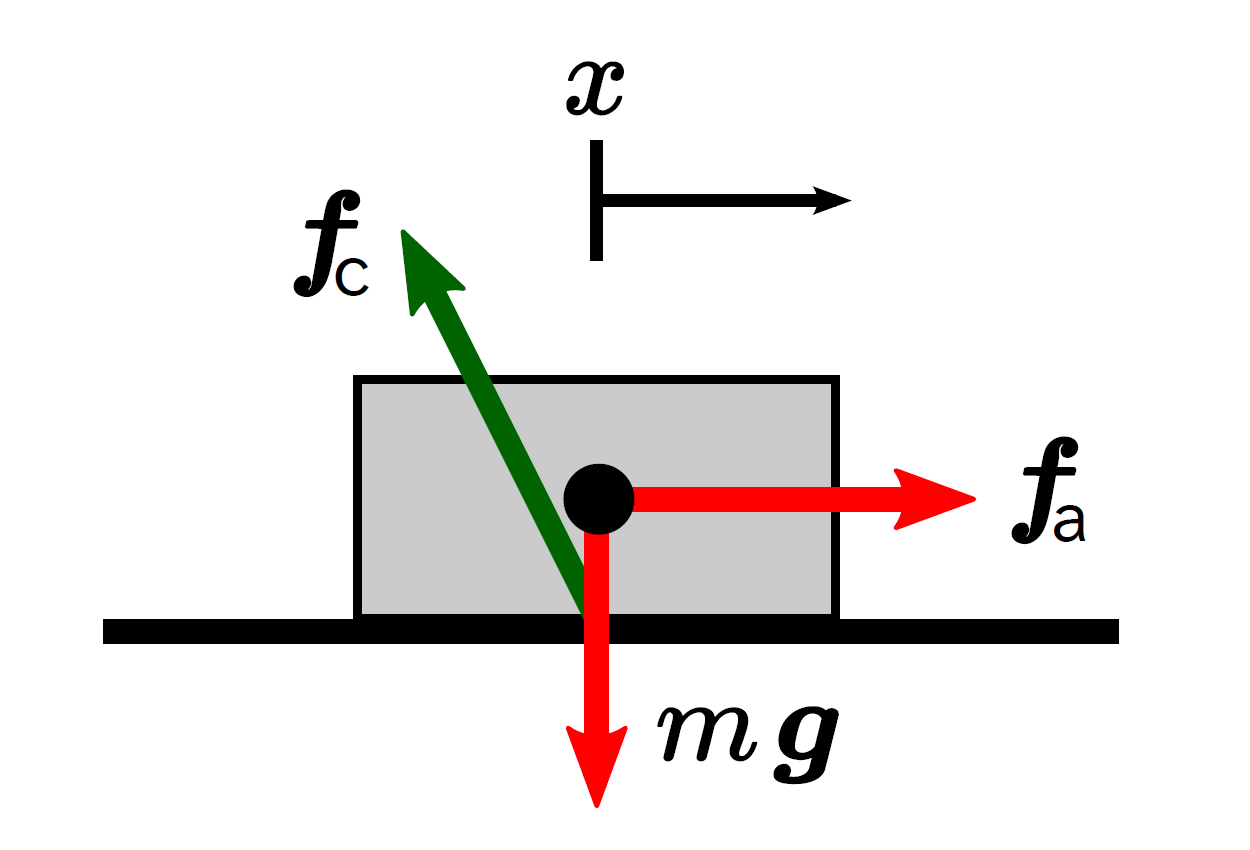
\includegraphics[width=.95\linewidth]{img/simple_contact}
		\caption{}
		\label{img:simple_contact}
	\end{subfigure}%
	\begin{subfigure}{.5\textwidth}
		\centering
		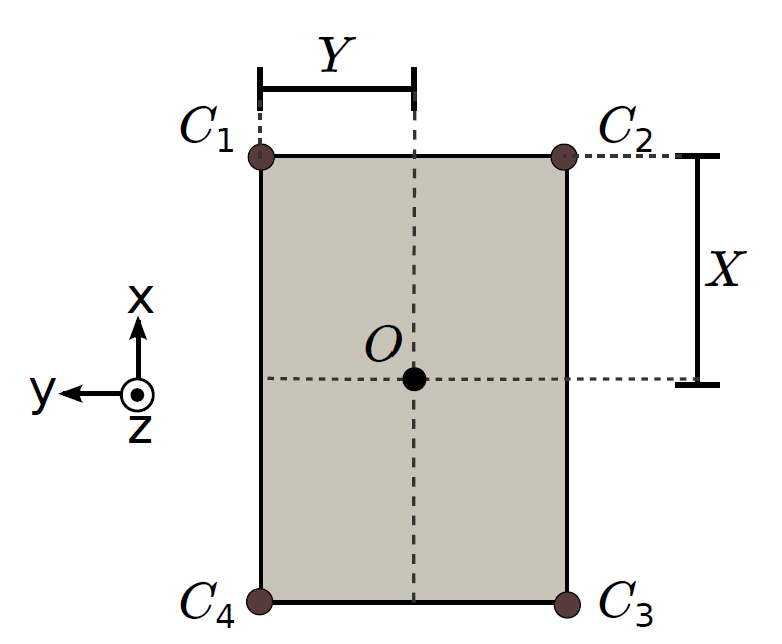
\includegraphics[width=.77\linewidth]{img/contact_surface}
		\caption{}
		\label{img:contact_surface}
	\end{subfigure}
	\caption[Simplified contact situation and CoP notation]{(a) Visualization of acting forces on a simple rigid body and (b) notation used for the \gls{CoP} definition in the contact surface plane \cite{caron2015stability}.}
	\label{fig:natural2robot}
\end{figure}


\section{Center of Pressure (CoP) Constraints}\label{sec:StabilityCoP}
In this section we will derive a universal set of implementable constraints that bound the \gls{CoP} to lie inside the rectangular contact area of each foot.

\subsection{CoP Stability Conditions}
Recapitulate the constraints from inequality \crefrange{subeqn:stabilityCoPPitch}{subeqn:stabilityCoPRoll}. Instead of using the absolute value of $X$ and $Y$, one can also formulate the constraints as
\begin{align}
\begin{split}
-X \leq C_x \leq X,\\
-Y \leq C_y \leq Y.
\end{split}
\end{align}
Based on this formulation it becomes evident that the \gls{CoP} is constrained to lie inside the foot geometry visualized in \cref{img:contact_surface}. In fact, these conditions can be represented via four single inequality equations as
\begin{align}\label{eqn:CoPInequalities}
\begin{split}
X + C_x \geq 0, \\
X - C_x \geq 0, \\
Y + C_y \geq 0, \\
Y - C_y \geq 0. \\
\end{split}
\end{align}
These four inequality equations will be used in the following to formulate the \gls{CoP} constraints.   

\subsection{CoP Computation}
Our goal is to determine explicit expressions for $C_x$ and $C_y$ for arbitrary floor orientations, including inclined ground. To this end, consider the computation routine for the \gls{CoP} from \cref{eqn:CoPComputation}
\begin{equation*} 
\bp_{CoP}=\dfrac{\bn\times\myM{\btau_O^c}}{\bfun^c\cdot\bn}.
\end{equation*}
For arbitrary orientations of the contact normal vector $\bn$, we obtain
\begin{equation}\label{eqn:CoPComputationDetailed}
\bp_{CoP}=\dfrac{\bn\times\myM{\btau_O^c}}{\bfun^c\cdot\bn} = \dfrac{\begin{bmatrix} n_x \\ n_y \\ n_z \end{bmatrix} \times \begin{bmatrix} t_x \\ t_y \\ t_z \end{bmatrix}}{\begin{bmatrix} f_x \\ f_y \\ f_z \end{bmatrix} \cdot \begin{bmatrix} n_x \\ n_y \\ n_z \end{bmatrix}} = 
\begin{bmatrix} n_yt_z - n_zt_y \\ n_zt_x-n_xt_z \\ n_xt_y-n_yt_x \end{bmatrix}\cdot \dfrac{1}{f_xn_x+f_yn_y+f_zn_y},
\end{equation}
and solve for the desired position $C_x$ and $C_y$ of the \gls{CoP} as
\begin{subequations}
\begin{align}
C_x&=\dfrac{n_yt_z - n_zt_y}{f_xn_x+f_yn_y+f_zn_y}, \label{subeqn:Cx}\\
C_y&=\dfrac{n_zt_x-n_xt_z}{f_xn_x+f_yn_y+f_zn_y} \label{subeqn:Cy}.
\end{align}
\end{subequations}

\subsection{CoP Inequality Constraints}
Now that we have found explicit expressions for computing the \gls{CoP} (\crefrange{subeqn:Cx}{subeqn:Cy}), we can insert them into \cref{eqn:CoPInequalities}, which gives a set of four \gls{CoP} constraints as 
\begin{align}\label{eqn:CoPInequalityEqs}
\begin{split}
X + \dfrac{n_yt_z - n_zt_y}{f_xn_x+f_yn_y+f_zn_y} \geq 0, \\
X - \dfrac{n_yt_z - n_zt_y}{f_xn_x+f_yn_y+f_zn_y} \geq 0, \\
Y + \dfrac{n_zt_x-n_xt_z}{f_xn_x+f_yn_y+f_zn_y} \geq 0, \\
Y - \dfrac{n_zt_x-n_xt_z}{f_xn_x+f_yn_y+f_zn_y} \geq 0. \\
\end{split}
\end{align}
These conditions can be written in matrix form as:  
\begin{equation}\label{eqn:CoPInequalityMatrix}
\begin{bmatrix}  
Xn_0 & Xn_1 & Xn_2 & 0 & -n_2 & n_1 \\
Xn_0 & Xn_1 & Xn_2 & 0 & n_2 & -n_1 \\
Yn_0 & Yn_1 & Yn_2 & n_2 & 0 & -n_0 \\
Yn_0 & Yn_1 & Yn_2 & -n_2 & 0 & n_0 \\ \end{bmatrix}
\begin{bmatrix} f^x \\ f^y \\ f^z \\ \tau^x \\ \tau^y \\ \tau^z \end{bmatrix} \geq
\begin{bmatrix} 0 \\ 0 \\ 0 \\ 0 \end{bmatrix},
\end{equation}
and finally yield an implementable set of inequality equations for constraining the \gls{CoP} to lie inside the rectangular contact area of each foot. 


\section{Integration Into the Crocoddyl Framework}\label{sec:StabilityIntegration}
This section presents the integration of the derived CoP inequality constraints from \cref{eqn:CoPInequalityMatrix} into the Crocoddyl framework. 

\subsection{Inequality Constraints by Penalization}
In \cref{sec:TheoryConstrainedDDP} we have discussed possible ways of incorporating inequality constraints into DDP-like solvers. Crocoddyl handles inequality constraints, such as joint limits or friction cone, via penalization. 
In numerical optimization, the goal is to minimize a given cost function. In Crocoddyl, an \textit{action model} combines dynamics and cost model for each knot of the discretized \gls{OC} problem from \cref{eqn:totalCost}. The cost function for an action model at knot $n$ can be written as: 
\begin{equation}\label{eqn:costSum}
l_n=\sum_{c=1}^{C}\alpha_c\Phi_c(\bq,\dot{\bq}, \btau), 
\end{equation}
where $C$ different costs $\Phi_c$ are weighted by a respective coefficient $\alpha_c\in R$. The goal of the following two parts is to demonstrate how the inequality \cref{eqn:CoPInequalityMatrix} is implemented inside a novel cost function into the framework.

\subsection{Computation of Residual and Cost}
%\subsection{Computation of the Residual}
In numerical analysis, the term \textit{residual} corresponds to the error of a result \cite{shewchuk1994introduction}. For the sake of compactness, we abbreviate \cref{eqn:CoPInequalityMatrix} as 
\begin{equation} \label{eqn:costPositive}
\myM{A} \myM{w} \geq \myM{0},
\end{equation}
where $\myM{A}$ corresponds to a matrix of \gls{CoP} inequality constraints and $\myM{w}$ is the contact wrench acting on the according foot. The residual $\myM{r}\in \myM{R}_{4\times 1}$ of the cost is retrieved by a simple matrix-vector multiplication:
\begin{equation}\label{eqn:costResidual}
\myM{r} = \myM{A} \myM{w}.
\end{equation} 

%\subsection{Computation of the Cost}
The residual vector depicted in \cref{eqn:costResidual} typically contains non-zero numbers. The resulting scalar \gls{CoP} cost value $\Phi_{CoP}$ is computed via a bounded quadratic activation as
\begin{equation}\label{eqn:CoPCostComputation}
\Phi_{CoP}=
\begin{cases}
\quad\dfrac{1}{2}\myM{r}^T\myM{r} &\mid \text{lb} = \myM{r} = \text{ub} \\[10pt]
\quad 0 &\mid \text{lb} \leq \myM{r} \leq \text{ub}.
\end{cases}
\end{equation}

In order to account for the positiveness of $\myM{r}$ (see \cref{eqn:costPositive}), the bounds are set to $\text{lb}=\myM{0}$ and $\text{ub}=\infty$, respectively. Finally, this bounded quadratic activation of the residual vector has the following implications:
\begin{itemize}
\item The \gls{CoP} cost is zero, whenever $\bp_{CoP}$ lies inside or on the border of the foot area spanned by $X$ and $Y$,
\item The \gls{CoP} cost increases in a quadratic manner, when $\bp_{CoP}$ exceeds the foot area spanned by $X$ and $Y$.
\end{itemize}  
Besides this formulation of the cost function also other designs are conceivable for the future. For example, the euclidean distance from the CoP to the coordinate origin could be considered when computing the residual (see  \cref{eqn:CoPCostComputation}).

\subsection{Basic Usage and Contributions}
%\subsection{Basic Usage of the CoP Cost}
The cost function is implemented in C++, but can be accessed via Python bindings for versatile and fast prototyping. In the following, a basic example is provided to demonstrate the interface of the \gls{CoP} cost function to the interested reader.
\begin{verbatim}
# 1. Creating the cost model container
costModel = crocoddyl.CostModelSum(state, actuation.nu)
# 2. Defining the CoP cost
footGeometry = np.array([0.2, 0.08]) # dim [m] of the foot area
CoPCost = crocoddyl.CostModelContactCoPPosition(state, 
crocoddyl.FrameCoPSupport(footId, footGeometry), actuation.nu)
# 3. Adding the CoP cost term with assigned weight to the cost model
costModel.addCost("LF_CoPCost", CoPCost, 1e3)
\end{verbatim}

%\subsection{List of Contributions}
The contributions of this thesis to the open-source framework Crocoddyl are summarized in two main pull requests. The first one, \href{https://github.com/loco-3d/crocoddyl/pull/792}{\#792} contains the basic formulation of the \gls{CoP} cost function for contact dynamics action models (see \cref{app:ContactCoP}). With \href{https://github.com/loco-3d/crocoddyl/pull/830}{\#830}, an additional version is added for the special case of impulse dynamics (see \cref{app:ImpulseCoP}).
A functional unit test that checks the cost against numerical differentiation as well as accessible python bindings can be found in the according directory of \cite{crocoddylweb}.


%\subsection{Backup: Friction Cone constraints}
%\begin{align}
%\begin{split}
%\mid\mid f^x\mid\mid &\leq \mu f^z \\
%\mid\mid f^y\mid\mid &\leq \mu f^z \\
%f^z &> 0
%\end{split}
%\end{align}
%For the case of four edges of the linear approximation of the friction cone, the equations become:
%\begin{equation}
%\begin{bmatrix} 1 & 0 & -\mu \\
%-1 & 0 & -\mu \\
%0 & 1 & -\mu \\
%0 & -1 & -\mu \\
%0 & 0 & -\mu \\ \end{bmatrix} \cdot
%\begin{bmatrix} f^x \\ f^y \\ f^z \end{bmatrix} \leq
%\begin{bmatrix} 0 \\ 0 \\ 0 \\ 0 \\ 0 \end{bmatrix}
%\end{equation}

%\subsection{CoP Constraints: Horizontal Floor}
%For the special case of horizontal floor, with the according normal vector $\myM{n}=[0,0,1]$, the \gls{CoP} can be computed with the help of \cref{eqn:CoPComputationDetailed} to 
%\begin{equation}
%\myM{p}_{CoP} = \begin{bmatrix} -t_y/f_z \\ t_x/f_z \\ 0 \end{bmatrix},
%\end{equation}
%which in turn can be represented by four inequality conditions:
%\begin{align}
%\begin{split}
%X-\dfrac{\tau_y}{f_z} &\geq 0, \\
%X+\dfrac{\tau_y}{f_z} &\geq 0, \\
%Y+\dfrac{\tau_x}{f_z} &\geq 0, \\
%Y-\dfrac{\tau_x}{f_z} &\geq 0. \\
%\end{split}
%\end{align}
%These conditions can be transformed into matrix form for the purpose of implementation as
%\begin{equation}
%\begin{bmatrix} 
%0 & 0 & X & 0 & -1 & 0 \\
%0 & 0 & X & 0 & 1 & 0 \\
%0 & 0 & Y & 1 & 0 & 0 \\
%0 & 0 & Y & -1 & 0 & 0 \end{bmatrix} \cdot
%\begin{bmatrix} f^x \\ f^y \\ f^z \\ \tau^x \\ \tau^y \\ \tau^z \end{bmatrix} \geq
%\begin{bmatrix} 0 \\ 0 \\ 0 \\ 0 \end{bmatrix}.
%\end{equation}




